In this section, we propose VARAN, a Variational Inference-based method for aggregating self-supervised speech model outputs. We begin by outlining the limitations of current approaches. We then explain how our method addresses them, provide its theoretical foundation, derive the training objective, and finally detail the resulting architectural changes to the model.

\subsection{Limitations of Current Aggregation Methods}\label{limitations}

A common approach for aggregating hidden states before applying the probing head for a any downstream task, as described in Section~\ref{sec:2_2}, introduces two key limitations: (1) an \textit{information bottleneck} resulting from compressing layer-specific features into a single vector $\hat{\boldsymbol{h}}$, and (2) a \textit{static layer prioritization}, where a fixed set of weights $w$ ignores the optimal combination of features $H$ that depends on the input $\boldsymbol{x}$.


\begin{figure*}[t!]
    \centering
    \begin{subfigure}[b]{0.241\textwidth}
        \centering
        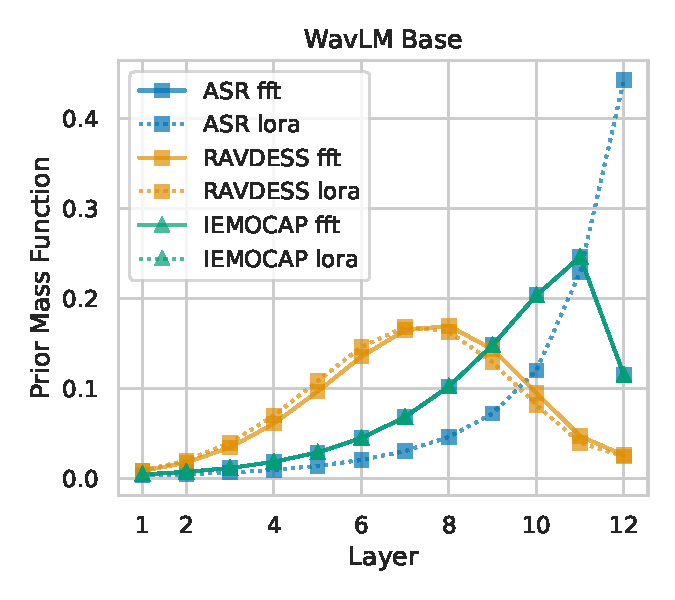
\includegraphics[height=1.2in]{figures/prior_wavlm_base.pdf}
    \end{subfigure}%
    ~ 
    \begin{subfigure}[b]{0.241\textwidth}
        \centering
        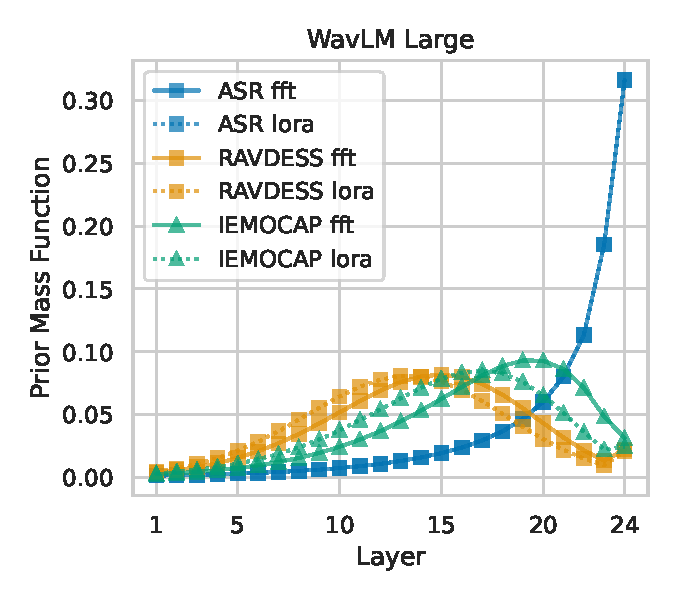
\includegraphics[height=1.2in]{figures/prior_wavlm_large.pdf}
    \end{subfigure}
    ~
    \begin{subfigure}[b]{0.241\textwidth}
        \centering
        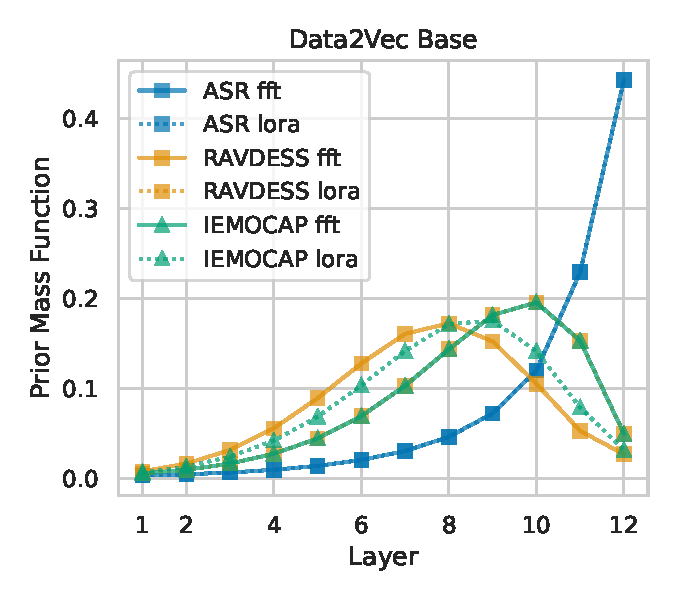
\includegraphics[height=1.2in]{figures/prior_data2vec_base.pdf}
    \end{subfigure}%
    ~ 
    \begin{subfigure}[b]{0.241\textwidth}
        \centering
        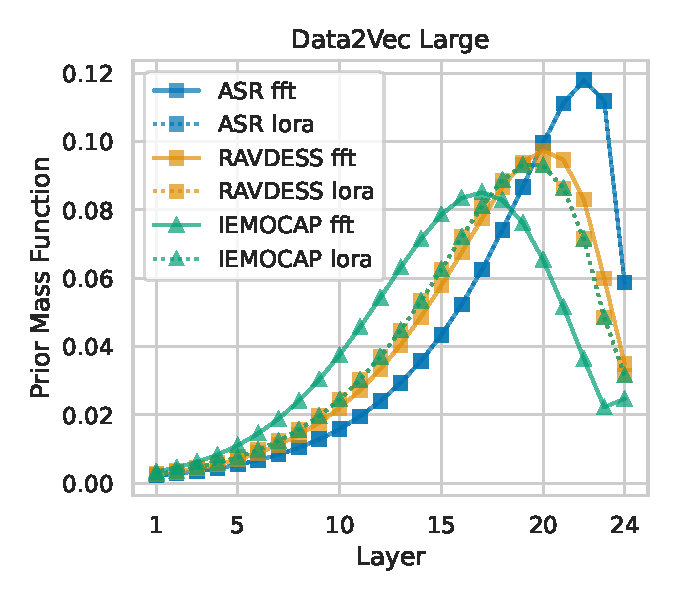
\includegraphics[height=1.2in]{figures/prior_data2vec_large.pdf}
    \end{subfigure}
    \caption{Prior distributions found during hyperparameters search. Models trained on RAVDESS\cite{livingstone2018ryerson} dataset tend to have distribution with mode on the middle layers. Models trained on ASR task (GigaSpeech \cite{DBLP:journals/corr/abs-2106-06909} dataset) in oposite tend to have distribution with mode on the last layer. See Section \ref{sec:analysis} for more details.} 
    \label{fig:prior}
\end{figure*}



\subsection{VARAN: Variational Inference Perspective}
To address the limitation of the existing layer aggregation methods we suggest to view a downstream task from variational inference perspective. We assume that for any downstream task, our goal is to predict the target $\boldsymbol{y}$ using input data $\boldsymbol{x}$. As mentioned in ~\ref{sec:2_2} one could use a simple linear classifier on top of the weighted sum of hidden layers, see Equation~\ref{eq:weighted_sum}, but we found this setup to be suboptimal, as it may require different layer weights $w$ to achieve the best performance for different tasks and even for individual samples. Choosing the right layer or combination of layers is challenging, as the training data does not have the optimal layer distribution.

However, we can learn it with the help of variational inference. In our setup, we have a classifier on top of each backbone's layer $p_\theta(\boldsymbol{y}\mid \boldsymbol{x}, l=i)$ and layer classifier $q_\theta(l \mid \boldsymbol{x})$, where $l$ is a discrete random variable and $i$ is a layer index. To maximize $p(\boldsymbol{y}\mid \boldsymbol{x})$, we can use the following objective:


\begin{align}
\label{eq:training_objective_vi}
L(\theta) &= - \mathbb{E}_{q_\theta(l \mid \boldsymbol{x})} \log p_\theta(\boldsymbol{y}\mid \boldsymbol{x}, l) \nonumber \\
&+ \operatorname{KL} \left(q_\theta(l\mid \boldsymbol{x}) \mid p(l)\right) 
\nonumber \\
&\geq - \log p(\boldsymbol{y}\mid \boldsymbol{x})
\end{align}

where $p(l)$ is a prior distribution on layer index. 

You can find more details on derivation in Appendix~\ref{appendix:elbo_deriviation}.

\subsection{VARAN: Training}
The training objective $L(\theta)$ derives from a variational upper bound, see Equation~\ref{eq:training_objective_vi}. Inspired by $\beta$-VAE \cite{higgins2017betavae}, we use a $\beta$ scaling factor as the regularization term. With this modification, our objective can be written as:
\cite{Kingma2013VAE}:  
\begin{align}
\label{eq:objective}
    L(\theta) &= - \mathbb{E}_{q_\theta(l \mid \boldsymbol{x})} \log p_\theta(\boldsymbol{y}\mid \boldsymbol{x}, l) \nonumber \\
    &+ \beta \operatorname{KL} \left(q_\theta(l\mid \boldsymbol{x}) \mid p(l)\right),
\end{align}
where the first term is a common downstream-task loss (eg. Cross Entropy for classification) computed for each $\psi_i(\boldsymbol{h}_i)$ and averaged with the predicted set of weighs $\{w_i(\boldsymbol{h}_i)\}_{i=1}^n$. 
Where $\psi_i$ is a probing head for each encoder layer $\mathbf{L}_i$.
Note that $\{w_i(\boldsymbol{h}_i)\}_{i=1}^n$ obtained individually for each sample $\boldsymbol{x}$.  Crucially, unlike Gumbel-based methods \cite{jang2016categorical}, gradients flow directly through $q_\theta(l|\boldsymbol{x})$, ensuring stable training of data-dependent weights.  

The second KL term regularizes the predicted distribution for each training sample toward a prior $p(l)$ defined for each downstream task. In practice, we used discretized reversed $\chi^2$ distribution and vary degrees of freedom during the hyperparameter search.

\subsection{VARAN: Inference}
At inference, predictions combine layer outputs via learned weights:  
\begin{align}\label{eq:inference}
    \log(\hat{p}(\boldsymbol{y}|\boldsymbol{x})) &= \sum_{i=1}^{n}q_\theta(l=i|\boldsymbol{x}) \cdot \log(p_\theta(\boldsymbol{y}|\boldsymbol{x}, l=i)) \nonumber \\  
    &= \sum_{i=1}^{n}w_i(\boldsymbol{h}_i) \cdot \log(\psi_i(\boldsymbol{h}_i)).  
\end{align}  


VARAN addreses both an information botteleneck and a static layer prioritization issues: the first component of Equation~\ref{eq:inference} ensures that the model learns a unique set of weights $w_i$ for each sample to enable flexible, dynamic feature integration. The second component overcomes the information bottleneck by introducing different probing heads $\psi_i$ that extract specialized information from each layer, incorporating these rich representations into the final output. 

\subsection{VARAN: Architectural Perspective}

An overview of the proposed method can be found in Figure~\ref{fig:varan}. To compute $q_\theta(l=i|\boldsymbol{x})$ the posterior distribution predictor is parameterized using Multi-Head Self-Attention (MHSA). The input to the MHSA consists of hidden states from the Transformer Encoder blocks $H = (\boldsymbol{h}_1, \dots, \boldsymbol{h}_n)$, where $\mathbf{h} \in \mathbb{R}^{\text{b} \times \text{s} \times \text{d}}$ (with dimensions corresponding to batch size $b$, sequence length $s$, and hidden size $d$). We apply mean pooling along the sequence length dimension and concatenate the results into a single tensor. This tensor is fed into the standard MHSA mechanism, which acts as a feature mixer across layers. 
Finally, we apply a linear layer to the last dimension to obtain a tensor $\mathbf{H_\text{projected}} \in \mathbb{R}^{\text{b} \times \text{L} \times 1}$, perform a squeeze operation to remove the singleton dimension and apply softmax function along the layer dimension to produce weights $\mathbf{w} \in \mathbb{R}^{\text{b} \times \text{L}}$ for each batch sample. To get $\log(p_\theta(\boldsymbol{y}|\boldsymbol{x}, l=i))$ we employ separate lightweight models $\psi_i$ for each output of the encoder layer $\boldsymbol{h}_i$ which in our implementation is a simple linear layer. The final vector is obtained using the weighted sum as in Equation~\ref{eq:weighted_sum}. The detailed implementation of the proposed method can be found at \url{https://github.com/deepvk/varan}.



\begin{table}[hb]
    \centering
    \begin{tabular}{@{} l| c c @{}}
        \toprule
        \multirow{2}{.0\linewidth}{Parameter} & \multicolumn{2}{c}{Values} \\ 
        \cmidrule(lr){2-3}
         & ASR & SER \\
        \midrule
        LoRa Rank & \{16\} & \{8, 16, 32\} \\
        Batch Size & \{16\} & \{16, 32, 64\} \\
        Weight Decay & \{0.1\} & \{0.05, 0.1\} \\
        Learning Rate & \{1e-5, 1e-4, 1e-3\} & \{3e-5, 1e-5, 1e-4\} \\
        KL $\beta$ & \{0.05\} & \{0.01, 0.05, 0.1\} \\
        $\chi^2$ DF & \{1, 3\} & \{3, 5, 15, 35, 50, 100, 400\} \\
        \bottomrule
    \end{tabular}
    \caption{Hyperparameter search space.}
    \label{tab:hp}
\end{table}



